\section{Recuperación de datos y formatos de serialización}
\subsection{Necesidad de formatos de serialización}
\begin{itemize}
\item Los formatos de \textbf{serialización} son vitales para el intercambio de datos
\item Más en el ámbito \textit{Big Data} (atacan a la "V" de la \textit{variabilidad})
\item A lo largo de los años se han diseñado formatos de serialización
\item Algunos son \textbf{más eficientes} que otros.
\item Algunos se han \textbf{estandarizado}.
\item En cualquier caso, son fundamentales para transmitir información, ya sea a través´s de \textbf{ficheros de disco} o bien para \textbf{comunicación por red}.
\item La mayoría de los formatos son \textbf{de propósito general}, por lo que una misma información se pude codificar \textbf{de varias formas} (por ejemplo, como \texttt{INSERT} en SQL, ficheros CSV, etc.)
\item Nuestro objetivo es conocer los formatos más usados para elegir el correcto en cada ocasión.
\end{itemize}
\subsection{Características a analizar}
\begin{itemize}[label=\color{lightblue}\textbullet,leftmargin=*]
	\item \textbf{¿Es un protocolo estándar?-} Con ello nos referimos a si está avalado por  cuerpo de estándares o su especificación 
	\item \textbf{¿Permite la codificación binaria?-} A la hora de transmitir grandes cantidades de información (ya sea en forma almacenada o bien a través de la red) es fundamental un protocolo binario para ahorrar espacio/tiempo.
	\item \textbf{¿Es legible por los humanos?-} A veces es interesante poder depurar un protocolo por parte de un humano. Esta idea comenzó con protocolos como XML, pero se ha ido abandonando porque no resulta muy factible salvo en ocasiones muy específicas.
	\item \textbf{¿Soporta referencias?-} A veces tenemos que relacionar partes de un conjunto de datos. Es interesante que los mecanismos de serialización permitan referenciar otras partes de un documento o de una comunicación.
	\item \textbf{¿Su estructura está definida por un Esquema o IDL?-} Al igual como sucedía con el lenguaje DDL de SQL, a veces es interesante que los datos sean conformes a algún esquema, también llamado IDL (\textit{Interface Definition Language}).
	\item \textbf{¿Es extensible?-} A veces es necesario acomodar datos que no se ajustan estrictamente a un esquema, o que son directamente no-estructurados.
	\item \textbf{¿Poseen un API estandarizado?-} Si los formatos de serialización poseen un API estandarizado será más sencillo no sólo compartir los datos, sino también compartir el código de serialización/deserialización (también llamado \textbf{marshalling})
\end{itemize}
\begin{itemize}[label=\color{red}\textbullet, leftmargin=*]
	\item \color{lightblue}Tabla resumen
\end{itemize}
\begin{tabular}{cccccccc}
\hline
 & Estándar & Bin? & Humano? & Ref? & IDL? & Ext? & API? \\
\hline
Apache Avro & Sí & Sí  & No & N/A & Sí (acoplado) & Sí & N/A \\
\hline
CSV & Parcial (RFC4180) & No & Sí & No & No & Parcial  & No \\
\hline
JSON & Sí (RFC7159) & No (BSON) & Sí & Sí (RFC6901) & Parcial  & Sí & No \\
\hline
Thrift & No & Sí & Parcial  & No & Sí (acoplado) & Sí & No \\
\hline
XML & Sí & Parcial & Sí & Sí & Sí & No & No \\
\hline
\end{tabular}
\subsubsection{Pandas}
\begin{itemize}
\item Pandas es una librería open source construida sobre \texttt{Numpy}.
\item Permite una preparación, limpueza y análisis rápido de los datos.
\item Una de sus principales características es la de visualización de datos.
\item Puede trabajar con una gran variedad de fuentes musicales.
\item Para instalar pandas es tan sencillo como ejecutar una de dichas instrucciones en el terminal \begin{center}
	\texttt{pip install pandas}\\
	\texttt{conda install pandas}
\end{center}
\bu{Dataframe}
\end{itemize}
\begin{itemize}
\item La herramienta más conocida y usada de Pandas son los \texttt{DataFrames}.
\item Permite almacenar datos tabulares en dos dimensiones similar a una hoja de cálculo o una base de datos relacional.
\item Las columnas de datos 
\end{itemize}
\begin{lstlisting}[language=Python]
df = pd.DataFrame(randn(5,4),index='A B C D E'.split(),columns='W X Y Z'.split())
\end{lstlisting}
\begin{verbatim}
	          W         X         Y         Z
	A -1.040684 -1.692150  1.707399 -1.257771
	B -0.403809 -1.024655  2.060558 -0.242150
	C -0.856354  0.173779  1.124053 -0.434952
	D  0.282316 -1.349518 -0.076797  1.077644
	E -0.152517 -0.603708 -0.812906  0.807102
\end{verbatim}
\subsubsection{XML (eXtensible Markup Language)}
\begin{itemize}
\item Meta-lenguaje de etiquetas derivado de SGML.
\item Motivación:
\begin{itemize}
\item Intercambio de datos en Internet
\end{itemize}
\item Reúne los requisitos de un lenguaje de intercambio de información:
\begin{itemize}
\item Simple: al estar basado en etiquetas y legible
\item Independiente de la plataforma: codificación UNICODE
\item Estándar y amplia difusión: W3C
\item Definición de estructuras complejas: DTD, Schemas
\item Validación y transformación: DTD, XSLT
\item Integración con otros sistemas
\end{itemize}
\item Facilita procesamiento lado cliente.
\item \textbf{No muy utilizado para BigData. Ha perdido tracción, es demasiado complejo finalmente y es muy poco eficiente en cual al porcentaje datos/metadatos}
\end{itemize}
\Ej
\begin{lstlisting}[language=XML, inputencoding=utf8, literate={Ñ}{{\~N}}1]
<?xml version="1.0" encoding="ISO-8859-1" ?>
<DISCO CODIGO="B000067FSG">
	<TITULO>Estrella de Mar</TITULO>
	<ARTISTA>Amaral</ARTISTA>
	<ESTILO>Pop</ESTILO>
	<REFERENCIA>
		<EDITORA>Virgin</EDITORA>
		<AÑO_EDICION>2002<AÑO_EDICION>
	</REFERENCIA>
	<MUSICOS>
		<MUSICO ROL="cantante">Amaral</MUSICO>
		<MUSICO ROL="guitarra">Juan Aguirre</MUSICO>
	</MUSICOS>
</DISCO>
\end{lstlisting}
\begin{itemize}
\item Instrucciones de procesamiento (línea 1)
\item Raíz (línea 2)
\item Etiquetas y atributos
\end{itemize}
\begin{itemize}[label=\color{red}\textbullet, leftmargin=*]
	\item \color{lightblue}DTD
\end{itemize}
\begin{lstlisting}[language=XML, inputencoding=utf8, literate={Ñ}{{\~N}}1]
<!ELEMENT DISCO (TITULO, ARTISTA, ESTILO?, REFERENCIA, MUSICOS)>
<!ATTLIST DISCO CODIGO ID #REQUIERED>
<!ATTLIST DISCO TIPO=(CD | LP | DVD) "CD">
<!ELEMENT TITULO (#PCDATA)>
...
<!ELEMENT REFERENCIA (EDITORA, AÑO_EDICION) >
<!ELEMENT MUSICOS (MUSICO*)>
...
\end{lstlisting}

Describe los documentos XML $\Longrightarrow$ \textbf{Validación}
\begin{itemize}[label=\color{red}\textbullet, leftmargin=*]
	\item \color{lightblue}DTD (ii)
\end{itemize}
Documento XML:
\begin{itemize}
\item \textbf{Válido:} sigue la estructura de un DTD
\begin{lstlisting}[language=XML, inputencoding=utf8, literate={Ñ}{{\~N}}1]
<!DOCTYPE web-app
	PUBLIC "-//Sun Microsystems, Inc.//DTD Web Application 2.2//EN"
	"http://java.sun.com/j2ee/dtds/web-app_2_2.dtd">
\end{lstlisting}
\item \textbf{Bien formado:} Sigue las reglas de XML
\end{itemize}
Limitaciones:
\begin{itemize}
\item No es XML
\item Tipado limitado de datos
\item No soporta espacios de nombres
\end{itemize}

\begin{itemize}[label=\color{red}\textbullet, leftmargin=*]
	\item \color{lightblue}Familias de estándares
\end{itemize}
\begin{itemize}[label=$-$]
	\item Schemas
	\begin{itemize}[label=\textbullet]
		\item Mismo propósito que un DTD, pero con mayor riqueza semántica.
		\item Sintaxis basada en XML.
		\item Contiene tipos predefinidos
		\item Espacios de nombres (\textit{namespaces})
	\end{itemize}
	\begin{lstlisting}[language=XML]
	<?xml version="1.0">
	<xsd:schema xmlns:xsd="http://www.w3c.org/2000/08/XMLSchema">
	<xsd:element name="Disco" type="DiscoTipo"/>
	<xsd:complexType name="DiscoTipo">
		<xsd:attribute name="codigo" type="String"/>
		<xsd:sequence>
		<xsd:attribute name="Titulo" type="String"/>
		<xsd:attribute name="Artista" type="String"/>
		<xsd:attribute name="Referencia" type="ReferenciaTipo"/>
		...
	\end{lstlisting}
	\item NameSpaces:
	\begin{itemize}[label=\textbullet]
		\item Espacios de nombres para cualificar elementos y atributos evitando la colisión de nombres.
		\item \texttt{xmlns:xsd="http://www.w3c.org/2000/08/XMLSchema"}
	\end{itemize}
	\item XSLT:
	\begin{itemize}[label=\textbullet]
		\item Definición de reglas de transformación de documentos
	\end{itemize}
	\item XSL:
	\begin{itemize}[label=\textbullet]
		\item Definición de hojas de estilos.
	\end{itemize}
	\item XPath:
	\begin{itemize}[label=\textbullet]
		\item Para hacer referencia a partes de un documento
		\item \texttt{/DISCO[Titulo="Estrella de Mar"], /DISCO//MUSICOS[1]}
	\end{itemize}
	\item XLink:
	\begin{itemize}[label=\textbullet]
		\item Enlace documentos entre sí.
	\end{itemize}
	\item XPointer:
	\begin{itemize}[label=\textbullet]
		\item Enlace de secciones dentro de un documento.
	\end{itemize}
	\item XQuery:
	\begin{itemize}[label=\textbullet]
		\item Consultas XML.
	\end{itemize}
\end{itemize}

\begin{itemize}[label=\color{red}\textbullet, leftmargin=*]
	\item \color{lightblue}Parsers
\end{itemize}
\begin{itemize}
	\item API SAX:
	\begin{itemize}
		\item Acceso secuencial al documento 
		\item Modelo de programación basado en eventos (\textit{callbacks})
		\item Simple y rápido: consume pocos recursos.
		\item Sólo consulta.
	\end{itemize}
	\item API DOM:
	\begin{itemize}
		\item Construye una estructura arbórea a partir del documento
		\item Potente, pero más costoso.
		\item Permite actualizaciones.
		\item Ideal para estructuras complejas.
	\end{itemize}
	\item En Python, existen numerosas formas de poder leer documentos XML.
\end{itemize}

\begin{itemize}[label=\color{red}\textbullet, leftmargin=*]
	\item \color{lightblue}API SAX
\end{itemize}

Librería \texttt{\textbf{xml.sax}}
\begin{lstlisting}[language=python]
import xml.sax

class XMLHandler(xml.sax.ContentHandler):
    def __init__(self):
        # Inicializamos variables de interés

    # Se llama cuando comienza un nuevo elemento
    def StartElement(self, tag, attributes):
        pass
    # Se llama cuando un elemento acaba
    def endElement(self, tag):
        pass

parser = xml.sax.make_parser()
parser.setFeature(xml.sax.handler.feature_namespaces, 0)
Handler = XMLHandler()
parser.setContentHandler(Handler)
parser.parse('models.xml') # nombre del documento a analizar
\end{lstlisting}
Cómo podríamos procesar con \texttt{\textbf{xml.sax}} este documento
\begin{lstlisting}[language=XML]
<collection shelf="New Arrivals">
    <model number="ST001">
        <price>35000</price>
        <qty>12</qty>
        <company>Samsung</company>
    </model>
    <model number="RW345">
        <price>46500</price>
        <qty>14</qty>
        <company>Onida</company>
    </model>
</collection>
\end{lstlisting}
\begin{itemize}[label=\color{red}\textbullet, leftmargin=*]
	\item \color{lightblue}Parser DOM
\end{itemize}
Librería \textbf{\texttt{xml.dom}}

\begin{minipage}{0.55\textwidth}
\begin{lstlisting}[language=python]
# Procesar un determinado fichero
file = minidom.parse('model.xml')

# Obtener los elementos con un determinado tag
modelos = fil.getElementosByTagName('modelo')

# Obtener el atributo 'nombre' del segundo modelo
print('modelo #2 atributos:')
print(modelos[1].attributes['nombre'].value)

# El datos de un item específico
print('\nmodelo #2 datos:')
print(modelos[1].firstChild.data)
\end{lstlisting}
\end{minipage}\qquad\begin{minipage}{0.4\textwidth}
\begin{lstlisting}[language=XML]
<data>
    <modelos>
        <modelo name='modelo1'>
            modelo1abc
        </modelo>
        <modelo name="modelo2">
            modelo2abc
        </modelo>
    </modelos>
</data>
\end{lstlisting}
\end{minipage}

\begin{itemize}[label=\color{red}\textbullet, leftmargin=*]
	\item \color{lightblue}Librería \texttt{BeatifulSoup}
\end{itemize}
\begin{minipage}{0.55\textwidth}
\begin{lstlisting}[language=python]
from bs4 import BeatifulSoup

# Leemos el fichero
with open('models.xml', 'r') as f:
    data = f.read()

# Pasamos los datos al parse
bs_data = BeatifulSoup(data, 'xml')

# Buscamos todas las instancias 'unique'
b_unique = bs_data.find_all('unique')
print(b_unique)

# Usamos .find búsquedas más concretas
b_name = bs_data.find('child', {'name':'Acer'})
print(b_name)
\end{lstlisting}
\end{minipage}\qquad\begin{minipage}{0.4\textwidth}
\begin{lstlisting}[language=XML]
<modelo>
    <child name="Acer" qty="12">
        Portátil Acer
    </child>
    <unique>
        Número de modelo
    </unique>
    <child name="Acer" qty="7">
        Exclusive
    </child>
    <unique>
        1.200€
    </unique>
</modelo>
\end{lstlisting}
\end{minipage}
\subsubsection{CSV (Comma-Separated Values)}
\begin{itemize}
\item Formato basado en columnas normalmente separado por coma
\item Sin embargo, el formato admite variaciones:
\begin{itemize}
\item Con o sin cabecera con los nombres de las columnas
\item Separador de columans (comas, tabuladores, etc.)
\item Codificación de caracteres (UTF-8, latin-1, etc.)
\item Escapado de caracteres (por ejemplo, una comilla doble como dos comillas dobles(" ") ó como \textbackslash")
\item Comillas opcionales (sólo si hacen falta) o en todos los campos siempre
\end{itemize}
\end{itemize}
\begin{itemize}[label=\color{red}\textbullet, leftmargin=*]
	\item \color{lightblue}Carga en SQL
\end{itemize}
\begin{lstlisting}[language=SQL]
LOAD DATA [LOW_PRIORITY | CONCURRENT] [LOCAL] INFLINE 'file_name'
    [RELACE | IGNORE]
    INTO TABLE tbl_name
    [PARCTITION (parctition_name, ...)]
    [CHARACTER SET charset_name]
    [{FIELDS | COLUMS}
        [TERMINATE BY 'string']
        [[OPTIONALL] ENCLOSED BY 'char']
        [ESCAPED BY 'char']
    ]
    [LINES
        [STARTING BY 'string']
        [TERMINATE BY 'string']
    ]
    [IGNORE number {LINES | ROWS}]
    [(col_name_or_user_var, ...)]
    [SET col_name = expr, ...]
\end{lstlisting}

\begin{lstlisting}[language=SQL]
LOAD DATA LOCAL INFILE "/tmp/Posts.csv"
    INTO TABLE Posts
    COLUMNAS TERMINATED BY ',' ENCLOSED BY '"' ESCAPED BY '"'
    LINES TERMINATED BY '\r\n'
    IGNORE 1 LINES;
\end{lstlisting}

\begin{itemize}[label=\color{red}\textbullet, leftmargin=*]
	\item \color{lightblue}Programación: Lectura con \texttt{Pandas DataFrame}
\end{itemize}
\begin{itemize}
	\item Lectura básica de un fichero CSV
	\begin{lstlisting}[language=python]
import pandas as pd
# Read the CSV file
airbnb_data = pd.read_csv("airbnb.csv")
	\end{lstlisting}
	\item Si queremos establecer la columna \lb{id} como índice
	\begin{lstlisting}[language=python]
airbnb_data = pd.read_csv("airbnb.csv", index_col="id")
	\end{lstlisting}
	\item Si queremos leer solo un conjunto de columnas
	\begin{lstlisting}[language=python]
usecols = ["id", "nombre", "barrio", "precio", "noches_minimias"]
airbnb_data = pd.read_csv("airbnb.csv", index_col="id", usecols=usecols)
	\end{lstlisting}
	\item Si queremos indicar un separador de columnas determinado
	\begin{lstlisting}[language=python]
usecols = ["id", "nombre", "barrio", "precio", "noches_minimias"]
airbnb_data = pd.read_csv("airbnb.csv", index_col="id", usecols=usecols, sep="|")
	\end{lstlisting}
	\item Si queremos definir el tipo de datos de determinadas columnas
	\begin{lstlisting}[language=python]
usecols = ["id", "nombre", "barrio", "precio", "noches_minimias"]
airbnb_data = pd.read_csv("airbnb.csv", index_col="id", usecols=usecols, sep="|", dtype:{'precio': float, 'barrio':str, 'noches_minimas':int}, decimal=',')
	\end{lstlisting}
\end{itemize}
\subsubsection{JSON (JavaScript Object Notation)}
Es, al mismo tiempo, un formato de archivo estándar abierto y un formato de intercambio de datos.\\
JSON se utiliza a menudo cuando los datos se envían desde un servidor a una página web.\\
En muchas ocasiones se define a JSON como \textit{autodescriptivo} y fácil de entender.

\begin{center}
	\includegraphics[scale=0.7]{"Temas/Tema 1/screenshot001"}
	
	\includegraphics[scale=0.7]{"Temas/Tema 1/screenshot002"}
	
	\includegraphics[scale=0.7]{"Temas/Tema 1/screenshot003"}
\end{center}
\begin{itemize}[label=\color{red}\textbullet, leftmargin=*]
	\item \color{lightblue}JSON Lines (JSONL)
\end{itemize}
\textit{JSON Lines} es un formato práctico para almacenar datos estructurados que pueden procesarse de uno en uno.\\
Ficheros con extensión \texttt{.jsonl}\\
Es un gran formato para archivos de registros.\\
Sigue las mismas convenciones que JSON salvo que el carácter \texttt{\textbackslash n} se usa como delimitador de líneas.\\
Cada línea de un fichero \texttt{.jsonl} es un JSON válido.

\begin{lstlisting}[language=json]
{"nombre": "Gilbert", "victorias": [["escalera"], ["pareja"]]}
{"nombre": "Alexa", "victorias": [["dobles parejas"], ["dobles parejas"]]}
{"nombre": "Maya", "victorias": []}
{"nombre": "Marisa", "victorias": [["trio"]]}
\end{lstlisting}

\begin{itemize}[label=\color{red}\textbullet, leftmargin=*]
	\item \color{lightblue}Lectura con \textbf{\texttt{Pandas DataFrame}}
\end{itemize}
\begin{itemize}
	\item Lectura básica de un fichero JSON
	\begin{lstlisting}[language=python]
import pandas as pd
df = pd.read_json('data.json')
	\end{lstlisting}
	\item Por defecto, Pandas sigue una orientación basada en columnas en la lectura de los ficheros \texttt{\{columna -> \{indice -> valor\}\}}
\begin{lstlisting}[language=python]
json_str = '{"Cursos":{"r1":"Spark"},"Tasas":{"r1":"25000"},"Duracion":{"r1":"50 días"}}'
df = pd.read_json(json_str)
print(df)
\end{lstlisting}
\begin{center}
	\begin{verbatim}
		   Cursos  Tasas Duracion
		r1  Spark  25000  50 días
	\end{verbatim}
\end{center}
\item Otras opciones son \texttt{index, records, split} y \texttt{values}.
\item Si usaramos la orientación records \dots
\begin{lstlisting}[language=python]
json_str = '[{"Cursos":"Spark","Tasas":"25000","Duracion":"50
	días","Descuento":"2000"}]'
df = pd.read_json(json_str, orient='records')
print(df)
\end{lstlisting}
\begin{center}
	\begin{verbatim}
		   Cursos  Tasas Duracion Descuento
		0   Spark  25000  50 días   2000
	\end{verbatim}
\end{center}
\item Estableciend el parámetro \texttt{lines} a \texttt{True}
\begin{lstlisting}[language=python]
df = pd.read_json('cursos.json', orient='records', nrows=2, lines=True)
\end{lstlisting}
\end{itemize}
\begin{itemize}[label=\color{red}\textbullet, leftmargin=*]
	\item \color{lightblue}Resumen
\end{itemize}
\begin{center}
	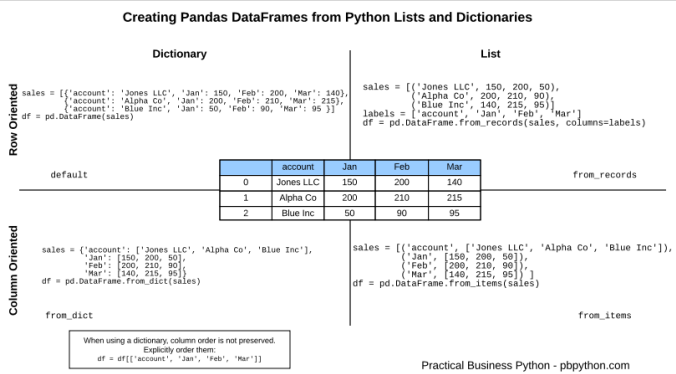
\includegraphics[width=0.7\linewidth]{screenshot001}
\end{center}
\subsubsection{Apache Avro}
Avro ofrece una serie de características:
\begin{itemize}
	\item Estructuras de datos ricas
	\item Un formato de datos compacto, rápido y binario
	\item Un lenguaje de especificación de esquema (Proto + IDL)
	\item Un formato de fichero contenedor para almacenar datos
	\item Un esquema de llamada a procedimiento remoto (RPC)
	\item Integración con lenguajes dinámicos, donde no hace falta recompilar el IDL (opcionalmente se puede hacer para lenguajes estáticos)
\end{itemize}
\begin{enumerate}[label=\arabic*)]
	\item Schema
\end{enumerate}
\begin{itemize}
	\item Una declaración de esquema se escribe en JSON. Bien un nombre de un objeto predefinido, o bien un objeto JSON de la forma:
	\begin{lstlisting}[language=python]
{"type": "nombreTipo", ... atributos ... }
	\end{lstlisting}
	\item Ofrece tipos primitivos y complejos. Primitivos: \texttt{null, boolean, int, long, float, bytes, string, . . .}
	\item \texttt{"{"type": "string"}"} es equivalente a "\texttt{string}".
	\item Tipos complejos permitidos: registros (records), enums, mapas, arrays, uniones.
	\item Tipos complejos: Récords (registros)
	\begin{itemize}
		\item El campo \texttt{type} se establece a \texttt{"record"}.
		\item El campo \texttt{name} establece su nombre.
		\item El campo \texttt{fields} establece sus campos. Cada campo:
		
	\end{itemize}
\end{itemize}